\documentclass[t]{beamer}

\input{../../../defs/preamble.tex}
\usecolortheme{crane}

\title[]{Experiment Design for Computer Sciences}
\subtitle[]{Introduction and Important Points}
\author[]{Claus Aranha\\{\footnotesize \url{http://conclave.cs.tsukuba.ac.jp/}}}
\institute{Computer Science Department}
\date{\scriptsize Tsukuba, 2017}

\begin{document}

\section{Introduction}
\subsection{Lecturer}
% cover page
\setbeamertemplate{footline}{}
\begin{frame}
  \titlepage
\end{frame}


% Main slides
\begin{ftst}
{Lecturer Introduction}
{Who am I?}
\begin{columns}[T]
  \column{0.4\textwidth}
  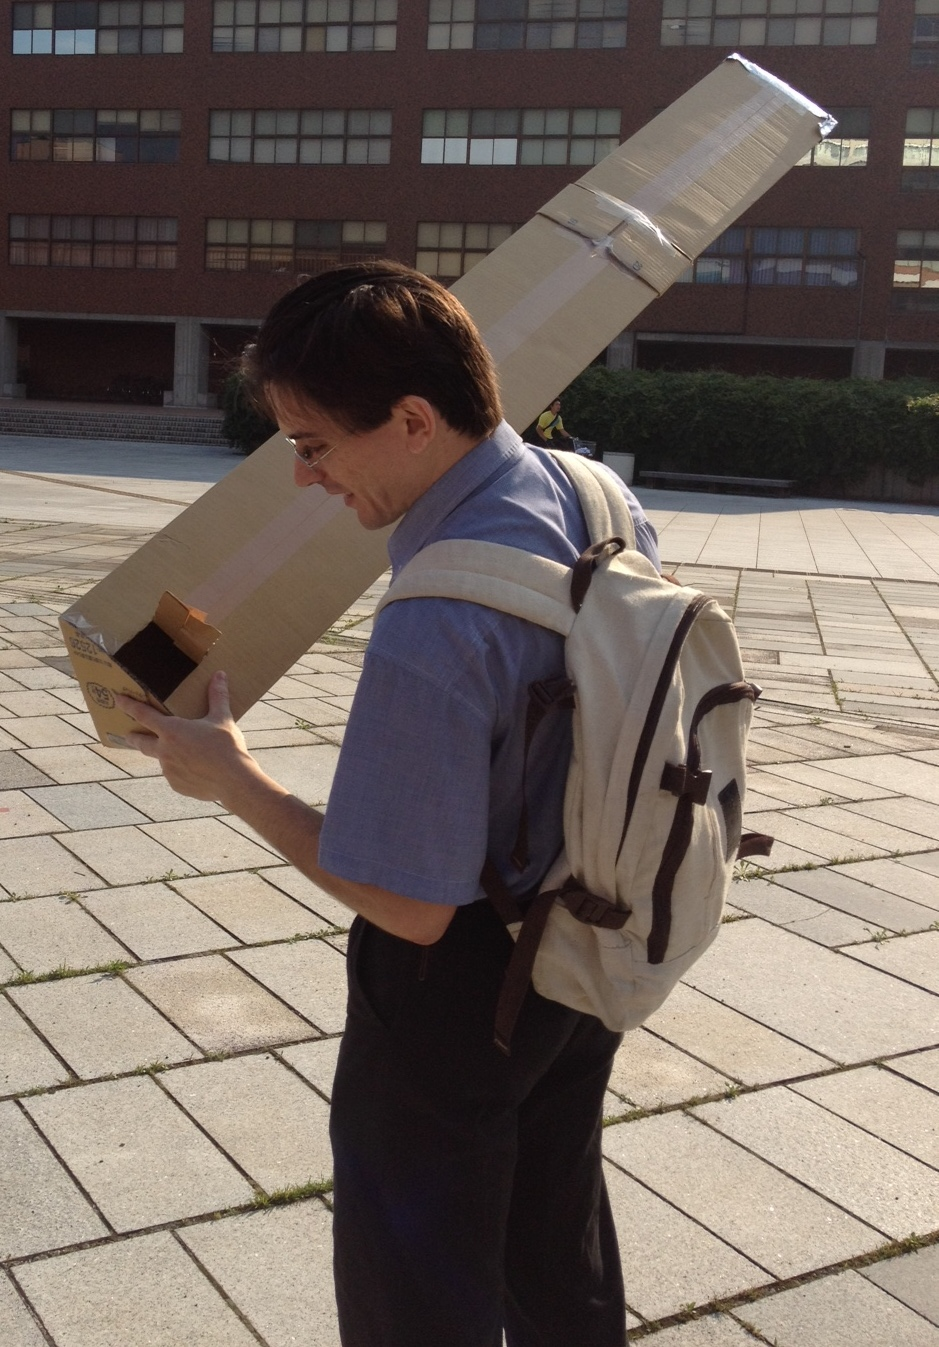
\includegraphics[width=1\textwidth]{../../../figs/pinhole}
  \column{0.6\textwidth}
  \bitems \structure{Name:} Claus Aranha;
  \item \structure{Country:} Brazil;
  \spitem \structure{Research:} Artificial Intelligence, Genetic
  Algorithms;
  \item \structure{Language:} R, Lua, Python, C++, Java;
  \item \structure{Hobbies:} Game Programming, Geocaching, Twitter
    Bots;

  \spitem \structure{Social Media (Twitter, Github):} \href{http://www.twitter.com/caranha}{@caranha}
  \eitem
\end{columns}
\end{ftst}

\subsection{Course Goals}

\begin{ftst}
  {Motivation}{Why is this course necessary?}  
  
  Many of you love maths, programming and technology. You want to
  create new gadgets and services. And now you are in your master
  degree.

  \hfill\includegraphics[width=.2\textwidth]{../../../figs/xkcd_science}
  
  Although there is a lot of overlap between the {\bf hacker} and the
  {\bf scientist}, there are some research related skills that many
  computer science students lack.\footnote{Julian Togelius has some
    nice insight about this different in
    see~\href{http://togelius.blogspot.jp/2016/04/the-differences-between-tinkering-and.html}{\color{gray}{\underline{this
          post}}}.}
  
  \vone

  The goal of this course is to introduce you to skills critical to
  perform scientific research (and which are nonetheless useful for
  engineering as well)
\end{ftst}

\begin{ftst}
  {Motivation}{A common example (1)\footnote{CC0 image from
      \href{https://pixabay.com/en/cat-pet-animal-cute-cat-cat-s-eyes-1360682/}{\color{gray}{\underline{pixabay}}}}}

  \begin{columns}[T]
    \column{0.80\textwidth}

    {\small You are a M1 student is studying neural networks to
      identify cat pictures. First, you use a common DNN structure
      from a web tutorial, and gets 90\% recall rate. Your advisor
      tells you need to create a {\bf novel} algorithm and a
      better result.}  \column{0.15\textwidth}
    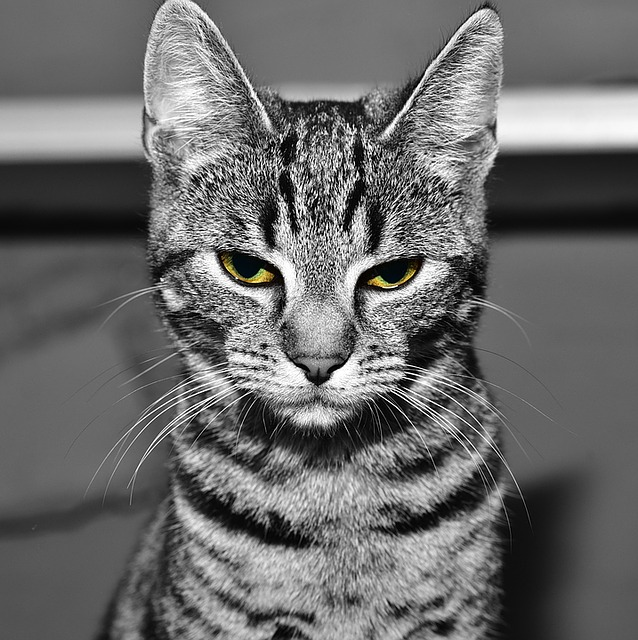
\includegraphics[width=1\textwidth]{../../../figs/cat}
  \end{columns}

  \vfill
  
  {\small

    You decide to try to use a polinomial as the activation function
    of a DNN (they are easy to derive...). After 5 months and a lot of
    trial-and-error, you get a 95\% recall rate with a 5-degree
    polinomial function! Yay!

    \vone

    Your advisor is happy, and you get a lot of positive feedback from
    the laboratory seminar. So now you try to publish you findings as
    a paper.

    \vone

    Everything perfect...}

\end{ftst}

\begin{ftst}
  {Motivation}{A common example (2)}

  {\small
    \begin{block}{Reviewer 1 (Major Revisions)}
      What is the sensitivity of your method to the parameters of the
      polinomial?
    \end{block}
    \begin{alertblock}{Reviewer 2 (Reject)}
      You need to perform an analysis of the significance of your
      experimentl result.
    \end{alertblock}
    \begin{alertblock}{Reviewer 3 (Reject)}
      Why did you use a 5 degree polinomial? Why not 4? Why not 7?
    \end{alertblock}
    \begin{exampleblock}{Reviewer 4 (Weak Accept)}
      You only use Tabby cat pics. What about siamese cats?
    \end{exampleblock}
    ... And, when you try to use siamese cat pictures, you get a 91\%
    recall!  }
\end{ftst}

\begin{ftst}
  {Motivation}{What happened?}

  The truth is that there is a big gap between hacking and
  science. The issues raised by the reviewers could have been
  preemptively solved by careful planning of the experiment:
  
  \vone

  \bitems What are the parts that can change, and to what limits?
\item How much can these changes affect the final result?
\item Which of these changes can be controlled, and which cannot?
\item If we control the changes, which values do we set?
\item How many times we test these different combinations?
  \eitem
  
  \vone
  
  Hacking relies on talent, determination and intuition. While science
  also needs these things, it also needs a lot of {\bf Careful
    Planning}.\footnote{CC0 image by jamonero from
    \url{https://www.openclipart.org}}

  \hfill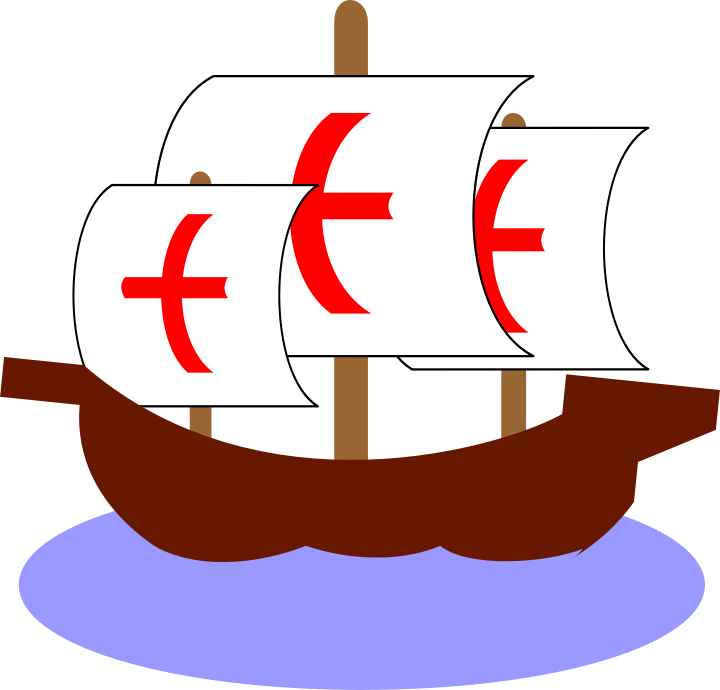
\includegraphics[width=.13\textwidth]{../../../figs/caravela}    
\end{ftst}

\begin{ftst}
  {Motivation}{In this course you will learn:}

\vfill
  
  \bitems The role of experimentation in the scientific method;

\vone
  
\item The principles of experimentalism;

  \vone
  
\item How to design an experiment, so you know what kind of result to
  expect before you start gathering data;

  \vone

  
\item The statistical tools for experiment data analysis and their
  mathematical background (with lots of examples)

  \vone
  
\item Some hints, tips and tricks on how to do SCIENCE!\eitem
\end{ftst}


\section{Technical Details}
\subsection{Grading}

\begin{ftst}
  {Grading System}{Or the part that everyone really wants to know (1)}
  This class is graded on a weighted average of four reports:

  \vone
  
  \begin{itemize}
  \item Mini-experiment (weight 1)
  \item Report on own research (weight 2)
  \item Case Study (weight 3)
  \item Experiment Report and Presentation (weight 4)
  \end{itemize}
\end{ftst}

\begin{ftst}
  {Grading System}{Or the part that everyone really wants to know (2)}
  \begin{block}{Mini-experiment -- Weight 1}
    Create a short, simple experiment based on his day to day
    experience, and submit a 1-page report on it by week 3.
  \end{block}
  \begin{block}{Report on your own research -- Weight 2}
    Write a short description of your research theme, indentifying
    what would be experimental parameters, sources of uncertainty, and
    describe a well designed experiment in your research following the
    themes of this lecture.
  \end{block}
\end{ftst}

\begin{ftst}
  {Grading System}{Or the part that everyone really wants to know (3)}
  \begin{block}{Case study -- Weight 3}
    Based on an experiment description and data provided by the
    instructor, write a report analysing the data properly using the
    methods discussed in class.
  \end{block}
  \begin{block}{Experiment, report and presentation -- Weight 4}
    Groups of two students must choose an experiment idea, design the
    experiment, perform the experiment, analyse the results and
    present their findings at the end of the semester.
  \end{block}
\end{ftst}

\subsection{Schedule}

\begin{ftst}
{Calendar}{}
\bitems 04/14 Week 1: What is Science? (Chapter 1)
\item 04/21 Week 2: The role of Experimentation (Chapter 2)
\item 04/28 Week 3: Basic Statistics (Chapter 3 and 4)
\item 05/05 \alert{Golden Week}
\item 05/12 Week 4: Hypothesis Testing (Chapter 5)
\item 05/19 Week 5: Comparisons (Chapters 6 and 7)
\item 05/26 Week 6: Non Standard Situations (Chapters 8 and 9)
\item 06/02 \alert{Week 7: Review and Case Studies}
\item 06/09 Week 8: ANOVA and multiple comparisons (Chapter 10)
\item 06/16 Week 9: Choosing Experiments (Chapter 11 and 12)
\item 06/23 Week 10: Final Review/Substitute Class
\item 06/30 \alert{Final Presentation}
\eitem
\end{ftst}

\subsection{Materials}

\begin{ftst}
  {Materials}{Reference Materials for this Course (1)}
  \begin{itemize}
  \item \alert{Design and Analysis of Experiments Repository}
  \item Manaba Online Classroom
  \item Books and Online Reads
  \end{itemize}

  \begin{block}{}
    Our main material for this course are the ``Design and Analysis of
    Experiments'' lecture notes, prepared and gracefully shared by
    Felipe Campelo from UFMG.

    \vone

    We will use a fork of this material that contains some extra information
    for Tsukuba, you can access it in this repository:

    \vone
    
    {\color{blue}\underline{{\small \href{https://github.com/caranha/Design-and-Analysis-of-Experiments}{github.com/caranha/Design-and-Analysis-of-Experiments}}}}
  \end{block}
  
\end{ftst}

\begin{ftst}
  {Materials}{Reference Materials for this Course (2)}
  \begin{itemize}
  \item Design and Analysis of Experiments Repository
  \item \alert{Manaba Online Classroom}
  \item Books and Online Reads
  \end{itemize}

  \begin{block}{}
    Copies of all PDFs, information about class structure, and Report
    submission will happen on the MANABA System. Please check
    freuently.

    \vone

    MANABA Page: \url{https://manaba.tsukuba.ac.jp/ct/course_754825}

    \vone
    
    Registration Code: \alert{5557872}
    
  \end{block}
\end{ftst}

\begin{ftst}
  {Materials}{Reference Materials for this Course (3)}
  \begin{itemize}
  \item Design and Analysis of Experiments Repository
  \item Manaba Online Classroom
  \item \alert{Books and Online Reads}
  \end{itemize}

  \begin{block}{}
    Each chapter in the Github has a list of required and suggested
    readings. These are usually quite short link, so be sure to read them!

    \vone
    
    In MANABA, there are lists for extra interesting links and videos
    not related to any one chapter in particular.
  \end{block}
\end{ftst}

\section{Expectations}
\subsection{Self Study}

\begin{ftst}
  {Expectations from the Students}{Self Study Requirements 1 -- Books}

  This course only convers a small (but significant~\footnote{pun
    intended}) part of D\&AoE techniques. In particular, each research
  might use slightly different methods depending on the type of
  experiments and data used.

  \vone

  Therefore, it is essential that you {\bf complement the classes with
    personal studies} from other sources. A good start is the course
  textbook:
  
  \vone

  \begin{itemize}
    \item D.C. Montgomery, Design and Analysis of Experiments, Wiley, 2005
  \end{itemize}

  \vone

  If you come across other material on the subject, feel free to
  recommend it to the rest of the class.
\end{ftst}

\begin{ftst}
  {Expectations from the Students}{Self Study Requirements 2 -- R Language}

  This course relies on many examples and case studies using the R
  language. It is {\bf essential} that you familiarize yourself with
  this tool.

  \vone

  \begin{center}
    \includegraphics[width=0.2\textwidth]{../../../figs/Rlogo}
  \end{center}
  
  \vone
  
  I recommend that you use the
  {\bf RStudio}\footnote{\url{https://www.rstudio.com}} IDE. Also,
  Coursera has regular {\bf tutorials on R
    programming}\footnote{\url{https://www.coursera.org/learn/r-programming/}}
  that can be easily completed in one or two weeks by anyone with
  familiarity in other programming languages.
  
  
\end{ftst}

\begin{ftst}
  {Expectations from the Students}{Self Study Requirements 3 -- English Language}

  {\bf Note:} writing clarity and correctness will count towards your
  grade. I don't expect any Shakespeare or Asimov, but {\bf reports
    consisting solely of code and figures} are not acceptable.

  \vone
  
  If you are not confident of your English abilities, professor Neil
  Millar\footnote{\url{mailto:millar@cs.tsukuba.ac.jp}} teaches the
  following courses for graduate level technical English:
  
  \vone
  
  \bitems Introductory Technical Writing: 02CA101
\item Advanced Technical Writing: 02CA103
\item Science Communication I: 02CA105
\item Science Communication II: 02CA107
  \eitem

  
\end{ftst}

\subsection{Behavior}

\begin{ftst}
  {Expectation from the Students}{Student Behavior 1 -- Attendance (or lack thereof)}

  I know that many of you will be busy with lab activities and your
  own research. I like to treat my students as responsible adults, so:

  {\small

  \bitems {\bf I do not take attendance for this course.} If you have to
  miss a class because of a lab meeting~\footnote{Or because Paradox
    released new DLC for EU4}, you have my blessings.
\item I am happy to answer questions about the course by e-mail, but
  discussions after class are much better for explaining complex
  topics.
\item Also, I am happy to discuss your personal research work,
  specially how to apply the contents of this course to your research.
\item I {\bf do expect} you to submit all assignments in time and
  participate in the final presentation.\eitem }
  
{\bf Make sure that you can afford to miss class!} If you don't come
to class and don't study the required readings, and don't ask me
questions, there is not much I can do to help you.

\end{ftst}

\begin{ftst}
  {Expectation from the Students}{Student Behavior 2 -- Plagiarism}

  \begin{center}
    \emph{Copying the work of one person is Plagiarism, Copying the work of many people is Research}
  \end{center}
  \hfill -- Graduate Proverb.

  \vone

  I take a {\bf very serious} view of plagiarism. Copying text or code
  from others without proper attribution will affect your grades and,
  in worse cases, may cause problems for your graduation.

  \vone

  On the other hand, (properly attributed) use of previous works, data
  and source codes is an important part of academic work, and
  encouraged. Don't reinvent the wheel.

  \vone

  \alert{When in doubt, don't hesitate to ask!}

\end{ftst}

\section{The end!}
\subsection{The end!}

\begin{ftst}
  {The End!}{Now let's get started}

  \begin{center}
    Questions?

    \vone

    Then Let's have fun! Time for the \alert{door of death...}
  \end{center}
\end{ftst}

\end{document}
